%% For double-blind review submission
\documentclass[acmsmall,10pt,review]{acmart}\settopmatter{printfolios=true}
%\documentclass[acmlarge]{acmart}\settopmatter{printfolios=false}
%% For single-blind review submission
%\documentclass[acmsmall,10pt,review]{acmart}\settopmatter{printfolios=true}
%% For final camera-ready submission
%\documentclass[acmsmall10pt,]{acmart}\settopmatter{}

%% Note: Authors migrating a paper from PACMPL format to traditional
%% SIGPLAN proceedings format should change 'acmsmall' to
%% 'sigplan'.


%% Some recommended packages.
\usepackage{booktabs}   %% For formal tables:
                        %% http://ctan.org/pkg/booktabs
\usepackage{subcaption} %% For complex figures with subfigures/subcaptions
                        %% http://ctan.org/pkg/subcaption

\usepackage{amsmath}

\newcommand{\cL}{{\cal L}}
\let\terms\undefined


\makeatletter\if@ACM@journal\makeatother
%% Journal information (used by PACMPL format)
%% Supplied to authors by publisher for camera-ready submission
\acmJournal{PACMPL}
\acmVolume{1}
\acmNumber{1}
\acmArticle{1}
\acmYear{2017}
\acmMonth{1}
\acmDOI{10.1145/nnnnnnn.nnnnnnn}
\startPage{1}
\else\makeatother
%% Conference information (used by SIGPLAN proceedings format)
%% Supplied to authors by publisher for camera-ready submission
\acmConference[PL'17]{LIVE Workshop}{}{}
\acmYear{2017}
\acmISBN{978-x-xxxx-xxxx-x/YY/MM}
\acmDOI{10.1145/nnnnnnn.nnnnnnn}
\startPage{1}
\fi


%% Copyright information
%% Supplied to authors (based on authors' rights management selection;
%% see authors.acm.org) by publisher for camera-ready submission
\setcopyright{none}             %% For review submission
%\setcopyright{acmcopyright}
%\setcopyright{acmlicensed}
%\setcopyright{rightsretained}
%\copyrightyear{2017}           %% If different from \acmYear


%% Bibliography style
\bibliographystyle{ACM-Reference-Format}
%\bibliographystyle{acm}
%% Citation style
%% Note: author/year citations are required for papers published as an
%% issue of PACMPL.
\citestyle{acmauthoryear}   %% For author/year citations


\begin{document}

%% Title information
\title[]{Live Programming By Example}         %% [Short Title] is optional;
                                        %% when present, will be used in
                                        %% header instead of Full Title.
%\titlenote{with title note}             %% \titlenote is optional;
                                        %% can be repeated if necessary;
                                        %% contents suppressed with 'anonymous'
%\subtitle{Subtitle}                     %% \subtitle is optional
%\subtitlenote{with subtitle note}       %% \subtitlenote is optional;
                                        %% can be repeated if necessary;
                                        %% contents suppressed with 'anonymous'


%% Author information
%% Contents and number of authors suppressed with 'anonymous'.
%% Each author should be introduced by \author, followed by
%% \authornote (optional), \orcid (optional), \affiliation, and
%% \email.
%% An author may have multiple affiliations and/or emails; repeat the
%% appropriate command.
%% Many elements are not rendered, but should be provided for metadata
%% extraction tools.

%% Author with single affiliation.
\author{William T. Hallahan}
%\authornote{with author1 note}          %% \authornote is optional;
                                        %% can be repeated if necessary
%\orcid{nnnn-nnnn-nnnn-nnnn}             %% \orcid is optional
\affiliation{
  %\position{Position1}
  \department{Computer Science}              %% \department is recommended
  \institution{Yale University}            %% \institution is required
  }
\email{william.hallahan@yale.edu}          %% \email is recommended

%% Author with single affiliation.
\author{Mark Santolucito}
%\authornote{with author1 note}          %% \authornote is optional;
                                        %% can be repeated if necessary
%\orcid{nnnn-nnnn-nnnn-nnnn}             %% \orcid is optional
\affiliation{
  %\position{Position1}
  \department{Computer Science}              %% \department is recommended
  \institution{Yale University}            %% \institution is required
  }
\email{mark.santolucito@yale.edu}          %% \email is recommended

%% Author with single affiliation.
\author{Ruzica Piskac}
%\authornote{with author1 note}          %% \authornote is optional;
                                        %% can be repeated if necessary
%\orcid{nnnn-nnnn-nnnn-nnnn}             %% \orcid is optional
\affiliation{
  %\position{Position1}
  \department{Computer Science}              %% \department is recommended
  \institution{Yale University}            %% \institution is required
  }
\email{ruzica.piskac@yale.edu}          %% \email is recommended


%% Paper note
%% The \thanks command may be used to create a "paper note" ---
%% similar to a title note or an author note, but not explicitly
%% associated with a particular element.  It will appear immediately
%% above the permission/copyright statement.
%\thanks{with paper note}                %% \thanks is optional
                                        %% can be repeated if necesary
                                        %% contents suppressed with 'anonymous'


%% Abstract
%% Note: \begin{abstract}...\end{abstract} environment must come
%% before \maketitle command
\begin{abstract}
Programming by example is a powerful approach to program synthesis and has enjoyed particular success as an aid to novice programmers.
While the theoretical foundations of programming by example continue to expand the potential for synthesis, it remains a special use case tool.
Aside from the FlashFill tool embedded within Excel spreadsheets, programming by example is not used by everyday programmers.
This is in part due to the lack of a native interface to support this new paradigm of programming.
We propose using live programming to help novice programmers better understand examples as a mode of programming.
\end{abstract}


%% 2012 ACM Computing Classification System (CSS) concepts
%% Generate at 'http://dl.acm.org/ccs/ccs.cfm'.
\begin{CCSXML}
%<ccs2012>
%<concept>
%<concept_id>10011007.10011006.10011008</concept_id>
%<concept_desc>Software and its engineering~General programming languages</concept_desc>
%<concept_significance>500</concept_significance>
%</concept>
%<concept>
%<concept_id>10003456.10003457.10003521.10003525</concept_id>
%<concept_desc>Social and professional topics~History of programming languages</concept_desc>
%<concept_significance>300</concept_significance>
%</concept>
%</ccs2012>
\end{CCSXML}

%\ccsdesc[500]{Software and its engineering~General programming languages}
%\ccsdesc[300]{Social and professional topics~History of programming languages}
%% End of generated code


%% Keywords
%% comma separated list
\keywords{Programming By Example, Live Programming}  %% \keywords is optional


%% \maketitle
%% Note: \maketitle command must come after title commands, author
%% commands, abstract environment, Computing Classification System
%% environment and commands, and keywords command.
\maketitle

\section*{Cooperative Programming: Integrating Software Synthesis with the Live Paradigm}
\paragraph{Overview:} Live programming is an emerging paradigm that is promising a vast change in the techniques used to develop modern software. A live programming environment allows a programmer to immediately see the effects of changes to a program on its outputs and effectively eliminates the edit-run-debug cycle that dominates programming workflows today. Our work seeks to develop new synthesis techniques that make use of the real-time feedback loop provided by a live programming environment. We will develop a system that allows a user to track a set of examples and synthesize subroutines to fit that set. When combined with fault localization techniques, programmers will be able to quickly find incorrect sections of code and initiate repairs that leverage information gleaned from the provided examples. While current  development tools provide tangible benefits to programmers skilled enough to use them, we aim to develop an accessible, first-of-its-kind, \textit{cooperative programming} environment that provides feedback in the form of generating representative examples and allowing changes to the code to be made through adjustments to these examples.

\paragraph{Intellectual Merits:} There are several open-ended problems to explore, including:

\begin{itemize}
\item Create novel, real-time algorithms to synthesize code within a live programming environment.
\item Investigate methods to evaluate the quality of an example set and methods to produce high quality example sets for a given program.
\item Build a formal theoretical framework for synthesis in a feedback loop.
\item Integrate these developments in a unified environment for a modern, major programming language - namely, Haskell.
\end{itemize}

\paragraph{Broader Impact:} We believe that cooperative programming environments will increase programmer productivity while simultaneously lowering the barriers for entry for newcomers to computer programming. Approaches to such environments must be informed by the needs of programmers, for whom these systems are ultimately built.

\section{Synthesis in Live Programming}
\label{sec:goal}


Writing a program is a relatively static process: a programmer writes some code and, after a successful compilation, can observe and inspect its behavior. If the code does not actually implement the programmer's intentions, she can correct the program and repeat the process.

The live programming paradigm advocates a more dynamic programming cycle that allows the programmer to inspect and understand the code as it is written. While existing incarnations of live programming environments mainly focus on programs with graphical output, we propose creating a general-purpose live programming framework, which is based
on the programming by example paradigm. 

Programming by example (PBE)~\cite{cypher93,lieberman01,synasc12} is a synthesis technique that automatically generates programs that coincide with given examples. An example is specified as a tuple of input and output values. Given a set $S= \{(i_1, o_1),\ldots, (i_n, o_n)\}$ of input/output examples, the goal is to automatically derive a program $P$ such that for every $j$, $P(i_j) = o_i$. The success and impact of this line of work can be estimated from the fact that some of this technology ships as part of the popular Flash Fill feature in Excel 2013~\cite{flashFillPOPL}.

Instead of writing code, the user provides a list of relevant examples and the synthesis tool automatically generates a program. In this way, the examples can be seen as an easily readable and understandable specification. However, even if the synthesized program satisfies all the provided examples, it still might not correspond to the user's intentions. Examples are, by nature, an incomplete specification. We believe that a live programming environment is an ideal framework to address this issue. Since the program continuously interacts with the programming environment, the user can provide new examples that better illustrate her intentions, and a synthesized program can be refined with each new example. We call this approach {\emph{cooperative programming}}.

Overall, our framework should incorporate programming by example technology with
Haskell. A live programming environment is obtained through a standard
Haskell REPL (Read Evaluate Print Loop) paradigm. 

\noindent\fbox{%
    \parbox{\textwidth}{%
A small demo of our envisioned approach is available in the following video \\
$\qquad$\url{https://www.youtube.com/watch?v=w5aI3N4dq2w}.    }%
}

In this paper we outline the main research topics that such framework would need to address. 

One of the major questions is how to provide the ``best'' representative examples, 
which illustrate the programmer intentions. An approach that fits nicely
in the live programming environment is that there is a list of examples automatically
generated from the already written code. We believe that a programmer gains a better understanding of her code through observing its execution on a sequence of representative inputs. Thus, we propose extending the programming environment with an interface to explore the code's execution on a set of example input-output pairs. We plan to use a symbolic execution engine to derive these examples.  While there is some existing work on symbolic execution of Haskell, we are currently developing our own symbolic execution engine~\cite{contract, HallahanTAPAS17}.  This work is motivated by the desire for a very general framework, adaptable to a variety of purposes,  that covers a wider range of Haskell than past efforts.
In addition to the examples automatically found using symbolic execution, extra examples could be optionally provided by the developer. This could be seen as an advanced debugging tool that traces execution on several values in parallel. Fig.~\ref{fig:tool} depicts a prototype user interface of such a live programming environment.

\begin{figure}[h!]
\centering
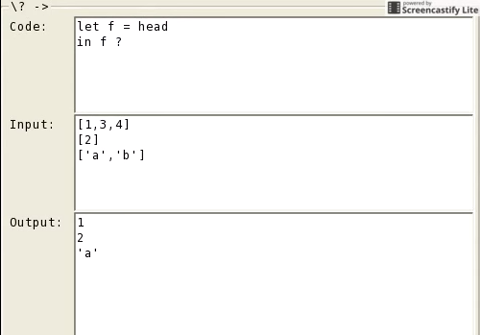
\includegraphics[scale=0.5]{tool}
\caption{A user interface for a live programming environment.}
\label{fig:tool}
\end{figure}

By observing changes in the input-output pairs, the user receives immediate feedback about whether the code is correct without actually analyzing it in detail. Any example that behaves unexpectedly acts as a real-time indication of an error in the code. 

The next question is how to correct the error? The user can go back to the code, detect
the source of the error and correct it manually. We, additionally, want to offer an 
automated repair by integrating recent advances in the PBE paradigm into this framework.
If the user notices that the current program for an input value $i$ returns an incorrect value $o$, then she can adjust that value to specify that her intended program should return $o'$ instead. This feedback could allow a tool to automatically synthesize a program which coincides with all given examples (included the modified ones) and which follows the structure of the original code as closely as possible.


\section{Research Questions Raised in Cooperative Programming }

To successfully develop the whole cooperative programming framework, 
we need to answer the following questions:
\begin{itemize}
\item How can we effectively represent the program to aid reasoning?  As previously mentioned, we plan to use symbolic execution to explore the possible inputs.  However, a major challenge here is scalability- a well known problem for symbolic execution is path explosion.  To address this, we plan to explore a variety of techniques, including aggressive identification and pruning of unhelpful paths, and making use of method summaries to abstract complicated functions.
\item Which parts of the code need to be modified so that the change is minimal with respect to some metric? In \cite{jose2011cause, pavlinovic2014finding} 
an algorithm based on MaxSAT/MaxSMT is used to find suitable candidates for the part of code in need of change.
\item How do we efficiently produce a program from a set of examples?
%As we show in Sec.~\ref{sec:pbe} there are synthesis algorithms for some types of input/output examples. Our goal is to define a general framework for programming by example.
We plan to further study existing synthesis approaches: the current work on programming by example is focused either on type-driven synthesis, or on SAT / SMT solvers to prone the search space. We plan to investigate combination techniques, as well as entirely new algorithms for programming by example.
\item Once we have detected a source of inconsistency between the code and the given examples, and we have synthesized a correct separate code, how can we incorporate those changes so that the structure of the existing code changes as little as possible?
We have previously explored this topic in the context of firewalls~\cite{HallahanFMCAD17}.  In this work, we model firewalls as first order logic formulas, and find repairs for them, given examples of incorrectly routed packets.  We hope our experience from this work will be valuable in developing techniques for such repairs in more expressive programming languages.
%We outline our approach in Sec~\ref{sec:repair}.
\end{itemize}

We plan to extend programming-by-example technologies to fully integrate them with our live programming system. As Fig.~\ref{fig:tool} might indicate, we will develop this system in Haskell, following a long tradition of support that the Yale Computer Science Department provides for the Haskell language. To the best of our knowledge, this is the first time that these techniques will be fully integrated with a mainstream programming language.
%
%We are particularly interested in Haskell to make use of the rich type system to prune the search space more effectively. Supporting type classes, for example, would help eliminate a large class of candidates. Other GHC language extensions will be evaluated on a case-by-case basis. Some might make synthesis easier (Existential Quantification), but others might introduce significant additional complexity (Arrows, Template Haskell).

\iffalse

\subsection{Modularity}

Since our target is a real programming language, scalability plays a vital role. We therefore focus on one method of the program at a time, observe its behavior, and generate suitable examples. However, if the user wants to understand a larger logical code fragment, the examples generated for only one method will likely not illustrate the larger code's behavior well enough. By ``context'', we mean a fragment of the program that we aim to observe; when creating representative examples, the context is an important parameter.

Depending on the size of the context, parts of code in this context might need to be abstracted. The PI's ongoing work on verification of nested data structures will help in developing the right level of abstraction. In our previous work, we developed a separation-logic based tool for automated verification of linked data structures, such as lists and trees \cite{PiskacWZ14, tacasPiskacWZ14, PiskacWZ13}. When extending these results for formal verification of complex data structures, such as hash sets or B-trees (unpublished, ongoing work), we needed to abstract away certain parts once they were formally verified. We believe that applying similar abstraction techniques can help delivering more representative examples.

Haskell is a programming language with strong static typing. While Haskell's rich type system suggests a type-directed approach, the type-checking step necessitates checking all the parts of the program a given fragment references. So unless the fragment only calls code we know to be finished (not under synthesis), we cannot consider the fragment in a context isolated from the rest of the program. To address this issue, we compute method summaries, which make it easier to generate high-quality examples and to more easily correct the code. We plan to adapt an existing tool, HALO \cite{VytiniotisJCR13}, for translating Haskell programs into first-order logic formulas to use in our framework.

Type-directed synthesis is a strategy to prune the search space of candidate functions. Type-directed synthesis for simple inductively defined data types was introduced in \cite{poseraZ15}, but only leverages this simple type information. Although attempting to synthesize across the full feature-set of any modern programming language is impractical  -- C++'s template system is Turing-complete, for instance -- we believe we will be able to support at least the same subset of Haskell as HALO.
\fi

\section{Related Work}
\label{sec:live}

In 2012 Bret Victor gave a presentation \cite{bretVictorVideo} at the Canadian University Software Engineering Conference (CUSEC 2012), where he promotes the idea that ``creators need an immediate connection to what they create''. Today's programming practice is far from that ideal: we first write code, then we compile it, and only then can we test it. If we are not happy with our program's output, we debug, modify the code and repeat the process. Victor proposed a new approach to programming in his talk. Dubbed  {\emph {live programming}}, the approach would help programmers better understand the code that they are writing. Similar to WSIWYG text editors, their changes to their code would have immediately observable effects on its output. His influential talk sparked interest for live programming and led to a number of nicely annotated editors for live coding. However, in a follow-up paper \cite{victor2012} Victor stresses that the goal of live programming is not merely to have a have a fancy editor, but to help the developer better understand what the code is doing.

Live programming is not a new term: as a concept it has been popularly adopted in processing images and sound (under the name ``live coding'')\cite{mclean14}. However, the ideas of live programming have been present for a long time in the programming language literature under various different names. Hancock studied ``real-time programming'' \cite{HancockPhDThesis}, a live programming environment for helping children to learn how to program. His research was focused on developing a Logo-like programming environment for robotics. Hancock argues that ``the coordination of discrete and continuous process should be considered a central Big Idea in programming and beyond'' \cite{HancockPhDThesis}.

McDirmid, et. al. \cite{McDirmid13oopsla, BurckhardtFHMMTK13_PLDI, McDirmidE14} sparked renewed academic interest in live programming. Their approach combines editing and debugging to obtain the required level of interactivity and  feedback. However, the applications they consider are restricted to graphical user interfaces. They, too, claim that live programming is the direction that  future programming environments should follow: ``Live programming is emerging as the next big step in programming environments that will finally allow us to move beyond our Smalltalk-era IDEs into a more programmer-friendly future. However, existing live programming experiences are still not very useful - they dazzle us with live feedback but that feedback does not really help us write code!'' \cite{McDirmid13oopsla}.

Some forms of live programming are present in various programming environments under different names. These include interactive programming, just in time programming, conversational programming, and on-the-fly-programming. Perera \cite{Perera08Journal} introduces a programming model called ``declarative interaction'' where he develops  a philosophical model that should unify all the live programming concepts. A list of requirements that a system built on this model should support includes: (1) an interaction between code and data; (2) robustness: a program should be able to repair and reconfigure without restarting, (3) transparency: changes and updates in code behavior should be consistent with program semantics, and the system should be able to generate and provide provenance data explaining the changes; (4) modular: in order to ensure scalability of the approach, system interactions should be restricted within a given scope. However, this scope should be able to dynamically change. Despite his description of such a model, Perera concludes that we still ``lack a simple and coherent paradigm for building robust interactive systems''.

Such a system can help the user to write better code, and through continuous interaction the user will gain a more comprehensive understanding of their program. We believe that enriching a live programming paradigm with program synthesis concepts, such as programming by example, will accomplish all of the goals set by Perera's project.



%% Acknowledgments
\begin{acks}                            %% acks environment is optional
                                        %% contents suppressed with 'anonymous'
  %% Commands \grantsponsor{<sponsorID>}{<name>}{<url>} and
  %% \grantnum[<url>]{<sponsorID>}{<number>} should be used to
  %% acknowledge financial support and will be used by metadata
  %% extraction tools.
  This material is based upon work supported by the
  \grantsponsor{GS100000001}{National Science
    Foundation}{http://dx.doi.org/10.13039/100000001} under Grant
  No.~\grantnum{GS100000001}{nnnnnnn} and Grant
  No.~\grantnum{GS100000001}{mmmmmmm}.  Any opinions, findings, and
  conclusions or recommendations expressed in this material are those
  of the author and do not necessarily reflect the views of the
  National Science Foundation.
\end{acks}


%% Bibliography
\bibliography{proposal}




\end{document}
